\section{Summary}
This thesis evaluated the performance a machine learning network with two different backbone for the selection of "good" source data which is to be used for the training of transfer learning algorithms for bin picking applications at \ac{IPA}. The two backbones are the PointNet Autoencoder and the \ac{DGCNN}. This thesis also evaluated the performance of different clustering algorithms for the purpose of generating representative members of the dataset in hand which constitute as "good" source data. The clustering algorithms evaluated in this procedure are Kmedoids, \ac{HDBSCAN}, spectral clustering and agglomerative clustering. A new concept called multi-level \ac{HDBSCAN} algorithm is also proposed in this thesis keeping the limitations in tis use-case in mind which is re-iterated in the next section. 

\vspace{5mm}

The best performance is attained by the model with PointNet Autoencoder as backbone. Several hyperparameter tuning is performed to improve the performance of the model. Using this model had a plethora of benefits. The performance of the clustering algorithms on the output of this model is better as compared to both the existent network at \ac{IPA} and also the model with the \ac{DGCNN} backbone. The training time for this model is significantly lower which facilitated further hyperparameter-tuning resulting in improved results. 

\subsection{Limitations}
There are several challenges encountered during the course of the thesis work. Firstly, the dataset that had to be worked on is extremely large, i.e. it has 1 million samples. Working with large datasets is a challenge in itself. Furthermore, each sample had 2048 points in the point cloud of datapoints. This is essential for learning the features of the objects to eventually come up with accurate feature representation of the objects. But this also makes it a dataset with high dimensionality. This made handling the dataset even more difficult. To tackle such large dataset with individual sample having high dimensions, the concept of dimensionality reduction had to be incorporated. This resulted in additional time in the pipeline and also loss of information about the data to some extent. But this step is extremely necessary to achieve the final goal of the thesis. 

\vspace{5mm}

Another very obvious problem already existing in these type of tasks is evaluating the performance of the clustering algorithms in unsupervised learning paradigm. Though the availability of the \ac{DBCV} index helped this situation to some extent, it incorporated challenges of its own. Calculating the \ac{DBCV} score depended heavily on the number of features of the datapoints. In the presence of a large number of features, it is impossible to work with such high dimensional data. This is a primary reason why the concept of dimensionality reduction had to be used. Because of how the \ac{DBCV} algorithm works, evaluating the performance of the clustering algorithms while considering all the datapoints together is unfeasible. So the performance of the clustering algorithm had to be evaluated for a smaller subset of the dataset. This made it crucial to verify if the performance followed a similar trend even for higher number of datapoints and the results obtained while working with a smaller subset of the dataset is enough to derive logical conclusions. Thus, developing a evaluation metric that can be used to determine the performance of the clustering algorithms in the presence of large high dimensional unlabelled dataset is a research scope for further studies.

\vspace{5mm}

Delving deeper into the clustering algorithm it is evident that the \ac{HDBSCAN} algorithm has significantly better performance as compared to any other clustering algorithm. But it had a major drawback of not having any control on the ultimate number of clusters obtained in the end. To circumnavigate this issue, the idea of multi-level \ac{HDBSCAN} is proposed. This naturally degraded the \ac{DBCV} score to some extent because the least-dense region within a cluster is no longer more dense as compared to the region in-between clusters. But had 2 important benefits, it had a control on the ultimate number of representative objects of the dataset which is very crucial in the present use-case. Also often times, it is observed that even though the result of this algorithm is not up to the mark as of \ac{HDBSCAN} algorithm, it is still better or at  least comparable to the next best algorithm, i.e. the spectral clustering algorithm. Furthermore, another significant benefit of multi-level \ac{HDBSCAN} algorithm as compared to spectral clustering is that the latter takes significantly higher time to cluster such a large dataset as compared to the former. Even in evaluations recorded in section \ref{sec:experiments} it can be seen that the time taken by the spectral clustering algorithm is quite high as compared to any other algorithm. For example, where multi-level \ac{HDBSCAN} algorithm takes 0.8 seconds to cluster 1000 datapoints, spectral clustering takes 7.2 seconds for the same task. This phenomenon is even intensified when the number of samples increase from 1000 datapoints to 1 million datapoints. Spectral clustering takes roughly 20 days to form 175 clusters from the entire dataset, whereas the multi-level \ac{HDBSCAN} takes as less as 3 hours. This is because spectral clustering has a time complexity of $O(N^3)$ for a dataset with N objects. Also, it is observed that multi-level \ac{HDBSCAN} had better performance in most cases as compared to spectral clustering. Thus, it is inefficient to use such large clustering time for worse performance.

\subsection{Discussions}

\begin{figure}[t]
    \centering
    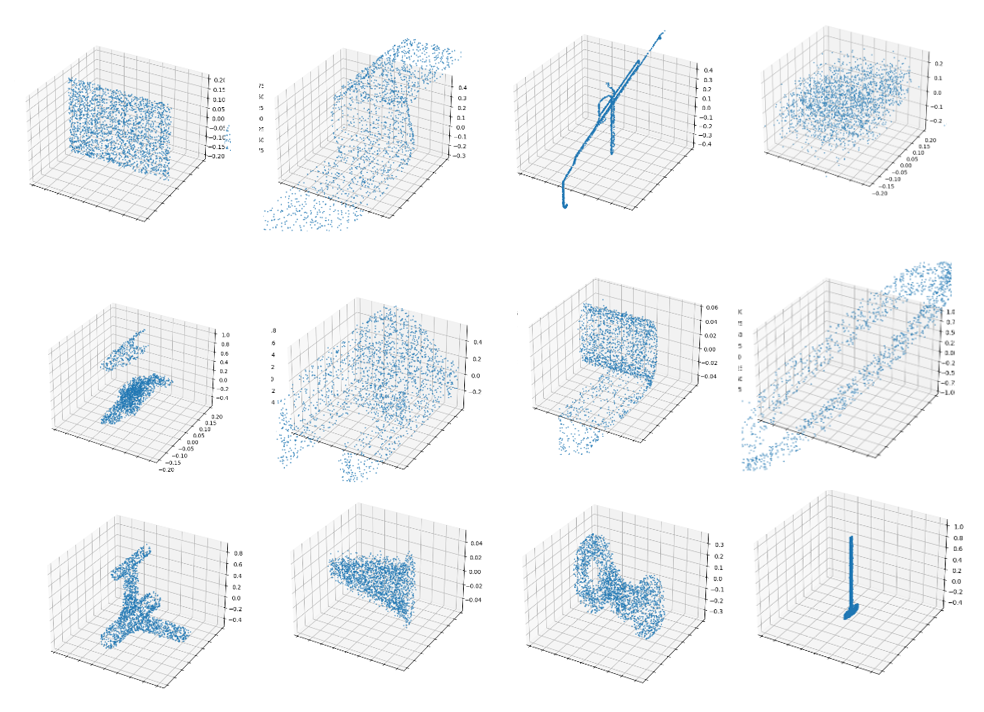
\includegraphics[width=400pt,height=300pt]{pictures/all_objs.PNG}
    \caption{Some of the representative members of the ABC dataset\cite{Koch_2019_CVPR} obtained on applying multi-level \ac{HDBSCAN} algorithm on the feature representations obtained from the ConClu approach with PointNet Autoencoder backbone.}
    \label{fig:all_hdbscan_objs}
\end{figure}

The ultimate goal of this thesis is to identify "good" source data that represents the variance of the entire dataset. It is observed that the objects obtained after the applying the clustering algorithms are quite diverse in nature. Although there is no known objective way to determine what qualifies as a "good" source object in case of unsupervised learning, the diversity in the objects obtained in the end quite ensures the fulfillment of the task in hand. Fig. \ref{fig:all_hdbscan_objs} shows some of the cluster representatives obtained after applying the multi-level \ac{HDBSCAN} algorithm. All the 175 representative members are included in the appendix. It can be seen that the representative objects of the dataset are quite diverse in nature. Thus, weighing the pros and cons of the two different backbones and the 5 different clustering algorithm, it can be concluded that the ConClu approach with the PointNet Autoencoder gives the best model for the generation of the latent space representations of te objects in the dataset. Furthermore, weighing the performance of the clustering algorithm under different setup and the overall time time required by the clustering algorithms, the multi-level \ac{HDBSCAN} algorithm seems to be a practical choice for this scenario. The \ac{HDBSCAN} algorithm has better performance compared to the multi-level \ac{HDBSCAN} algorithm because more number of clusters would naturally mean more smaller but dense clusters. But since it has no control on the number of clusters it returns and mostly returns a large number of clusters in the presence of a large dataset. Having such a high number of cluster representatives isn't feasible for further tasks in the current setup at \ac{IPA}. This is why the maximum number of cluster representatives is set to 175. Under this particular constraint, the multi-level \ac{HDBSCAN} algorithm is the best choice for clustering algorithm in this use-case. 

\subsection{Future Scope}

Finding a suitable clustering evaluation metric is a challenge by itself. Having a large high dimensional dataset increases the obstacles of it even more. So, finding a better evaluation metric for evaluating the performance of clustering algorithms is a research scope for further studies. Furthermore, it is seen that the performance of spectral clustering algorithm is often comparable to that of multi-level \ac{HDBSCAN} algorithm. But it required an impractical amount of time for the spectral clustering algorithm to converge. The hyperparameters in spectral clustering could be fine-tuned to evaluate if it ameliorates the convergence time. The values of certain parameters are set according to \cite{mei2022unsupervised}, specially in the  Sinkhorn-Knopp algorithm module. Better domain knowledge could possily improve the performance, if the hyperparameters are fine-tuned further. 